With our experiments we want to show three key results. The first result is that our virtual machine performs well when running multiple threads,
i.e., it can reasonably schedule the execution of programs to reduce execution time and increase parallel speedup. The second result is that by using coordination directives, programs perform faster. Third, we want to show that our programs are usually shorter than programs written in other languages.  

In our experimental setup, we used a machine with
four AMD Six-Core Opteron TM 8425 HE (2100 MHz) chips (24 cores) and 64 GB of DDR-2 667MHz (16x4GB) RAM,
     running GNU/Linux (kernel 2.6.31.5-127 64 bits).
     We compiled our virtual machine using GCC 4.4.5 (g++) with the flags \texttt{-O3 -std=c+0x -march=x86-64}.
     We run all experiments 3 times with the same configuration and then we averaged the run time.

\subsection{Parallel Experiments}

For the parallel results, we run each program using 1, 2, 4, 6, 8, 10, 12, 14 and 16 threads and compared the runtime against the execution of the sequential version of the virtual machine. We used the following programs:

\begin{description}
   \item[greedy graph coloring]: In this program, we attempt to color each node of a graph so that no two adjacent nodes have the same color. We start with 15 colors and expand the number of colors when we cannot color the graph.
   \item[pagerank]: The asynchronous PageRank algorithm without synchronization between iterations. Every time a node sends a new rank to its neighbors and the change was significant, the neighbors are scheduled to recompute their ranks.
   \item[N queens]: Already explained before. We use an 11x11 board.
\end{description}

In Fig.~\ref{exp:graph_coloring} we present the speedup results for the graph coloring program. In the first plot, we show the speedup for a graph of 12000 webpages. Since this dataset follows the power law, that is, there is a small number of pages with a lots of links (1\% of the nodes have 75\% of the edges), the speedup is not as good as the one shown when using a random dataset of 2000 nodes, where each node has more or less the same number of links. In the weather web graph 20\% of the nodes have 75\% of the edges, much less than the search engine dataset, and it shows in the results.

\newcommand{\figsize}[0]{5cm}

\begin{figure*}[htp]
   \centering
   \resizebox{\figsize}{!}{\subfigure[Using a search engine web graph (almost 12000 nodes)]{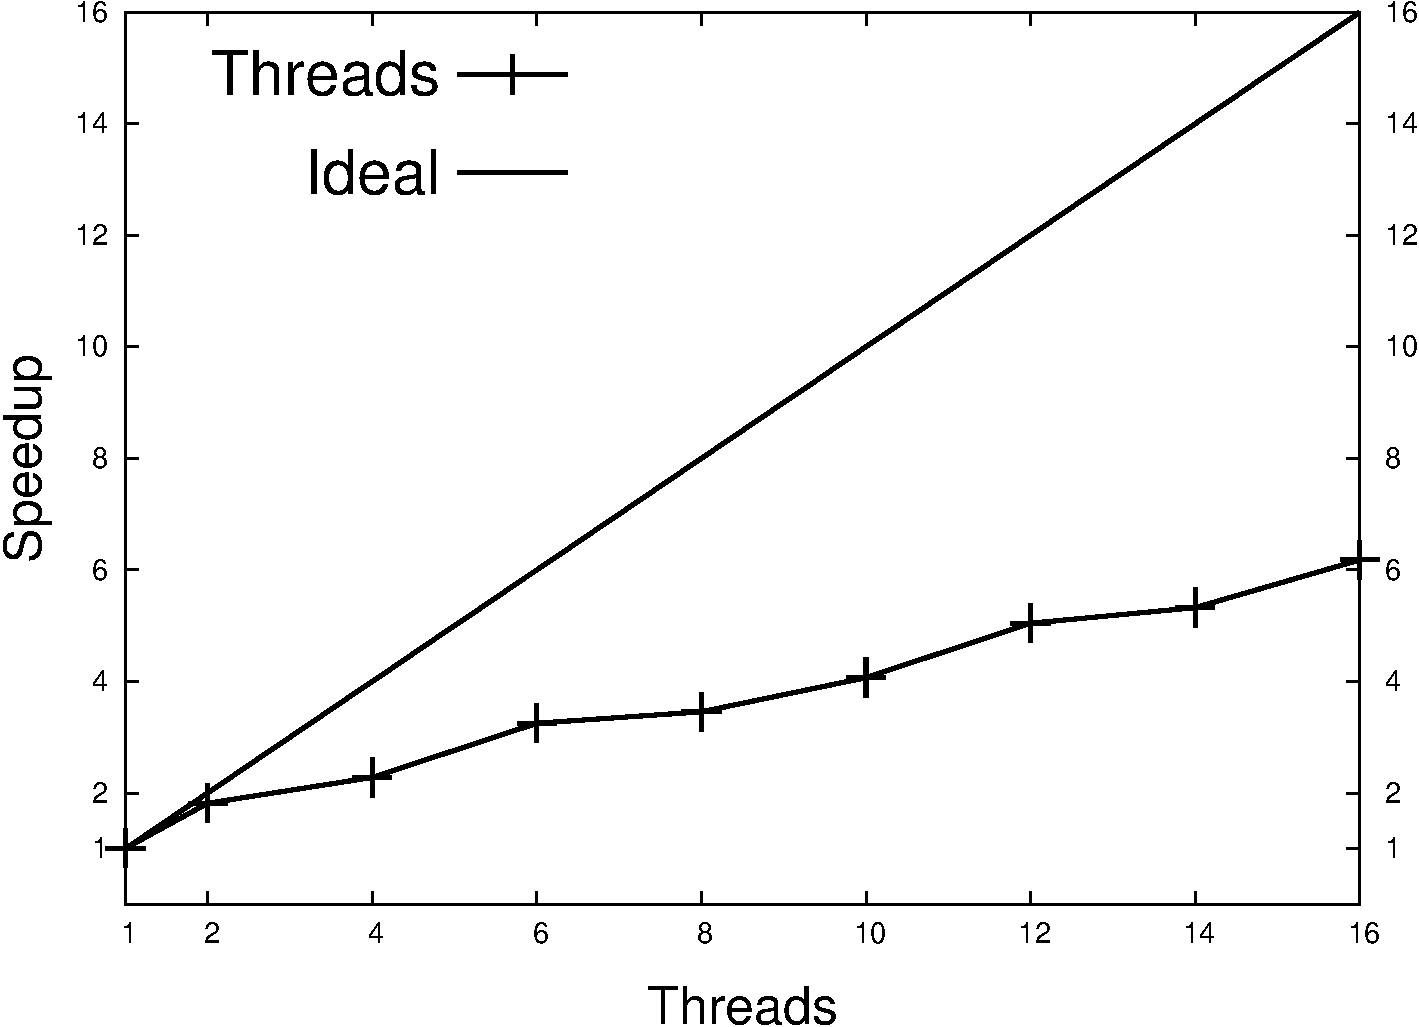
\includegraphics[width=0.5\textwidth]{speedup_greedy-graph-coloring-search_engines.pdf}}}
   \resizebox{\figsize}{!}{\subfigure[Using a weather web graph (around 8000 nodes)]{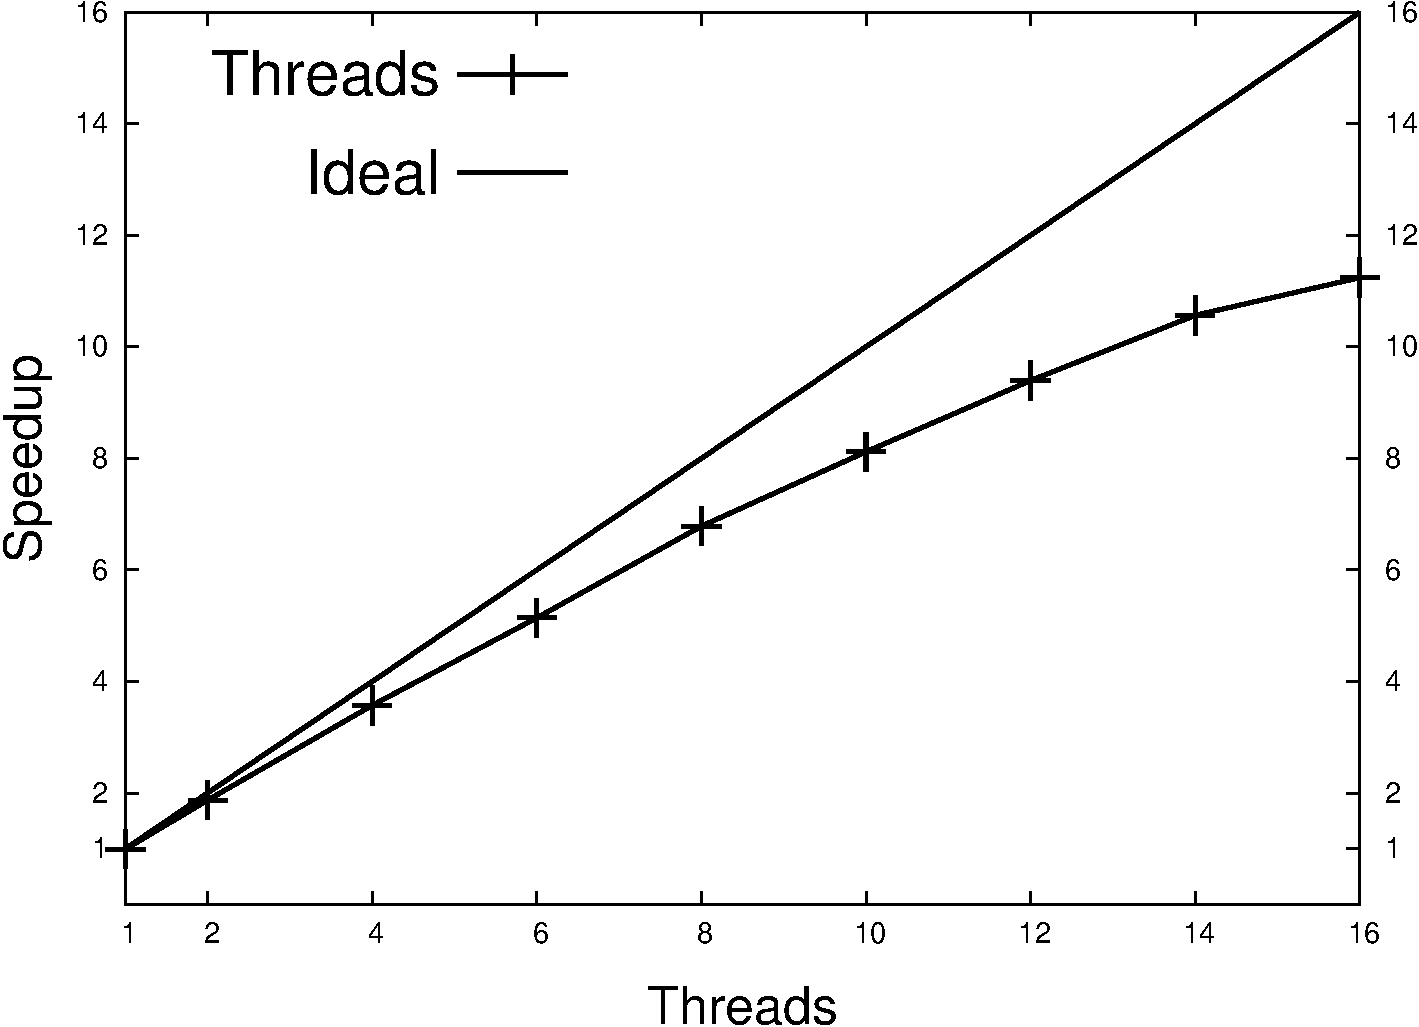
\includegraphics[width=0.5\textwidth]{speedup_greedy-graph-coloring-weather.pdf}}}
   \resizebox{\figsize}{!}{\subfigure[Using a random graph (with 2000 nodes)]{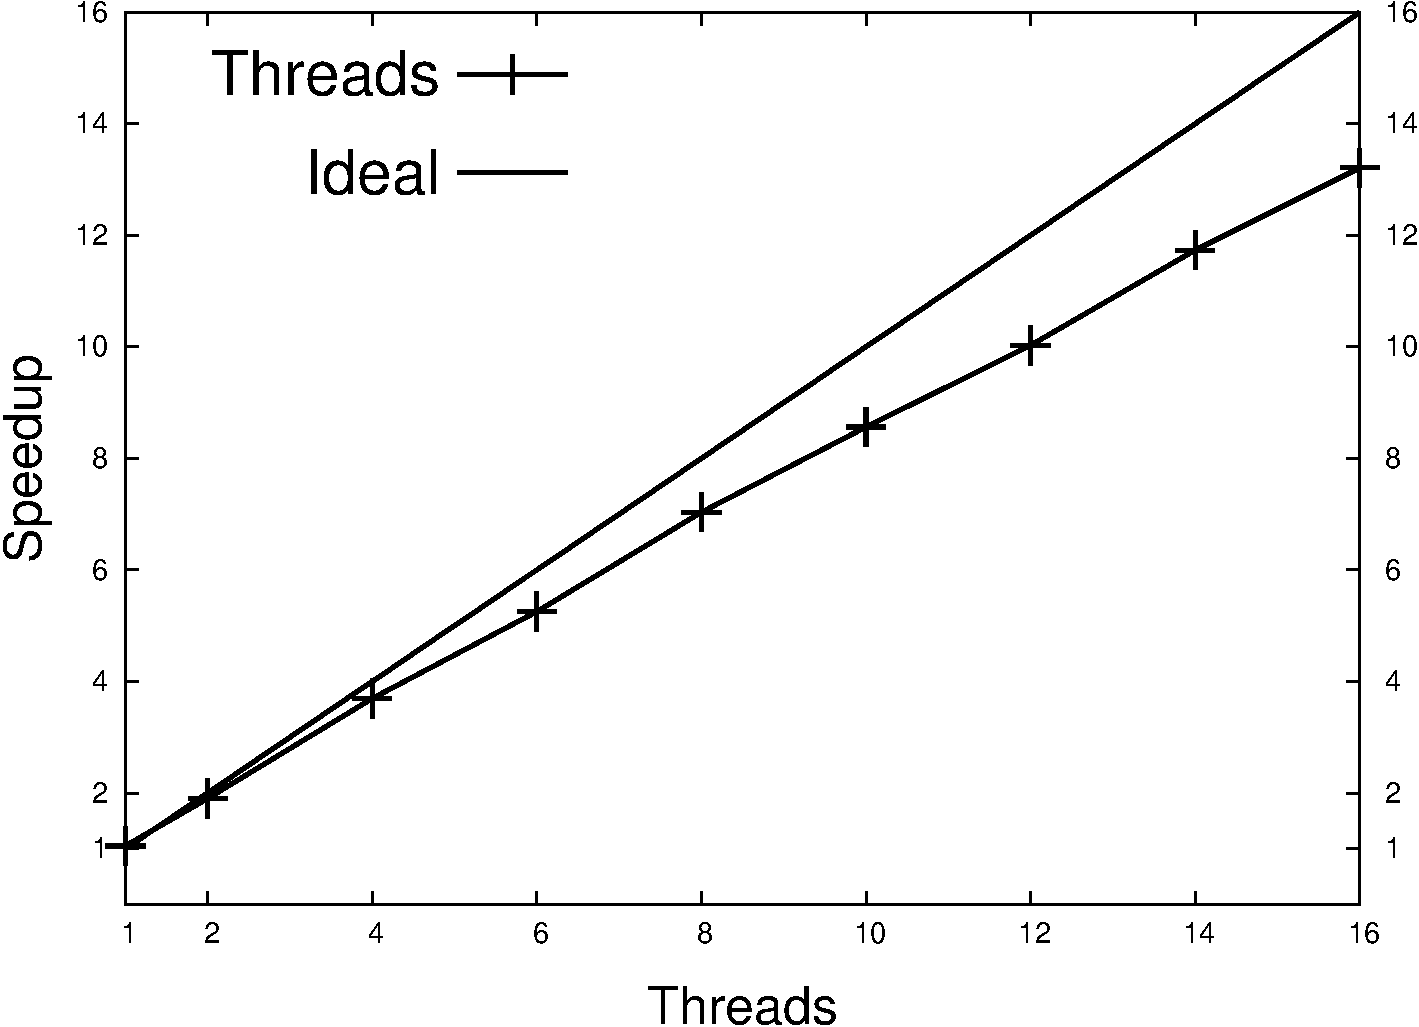
\includegraphics[width=0.5\textwidth]{speedup_greedy-graph-coloring-2000.pdf}}}
   \caption{Experimental results for the greedy graph coloring algorithm.}
   \label{exp:graph_coloring}
\end{figure*}

\begin{figure*}[htp]
   \centering
   \resizebox{\figsize}{!}{\subfigure[Using a search engine web graph (almost 12000 nodes)]{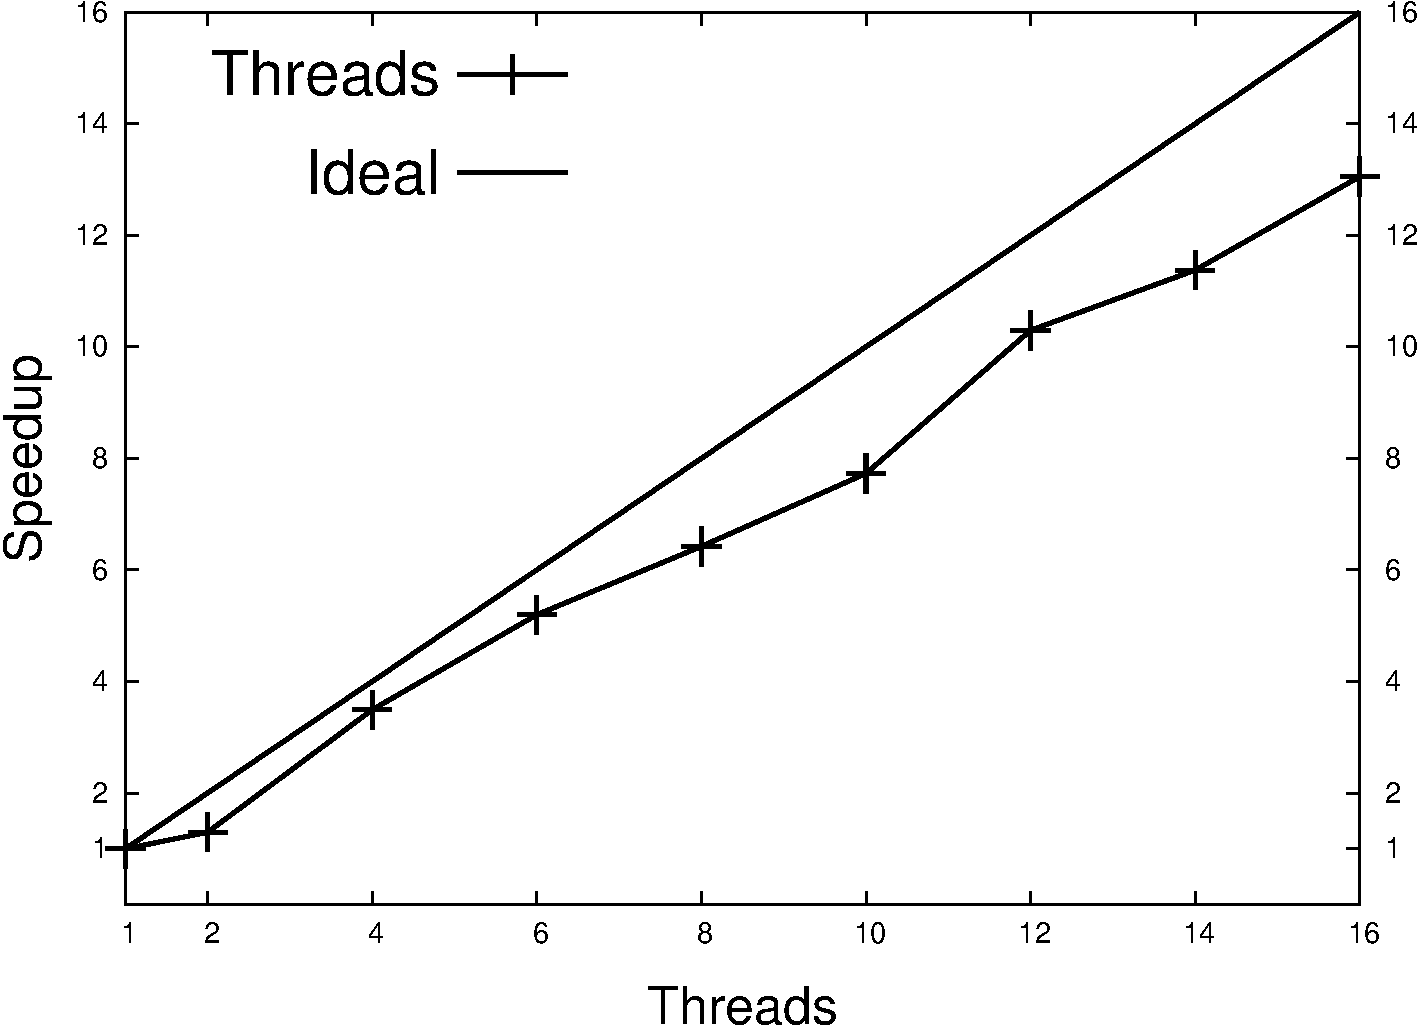
\includegraphics[width=0.5\textwidth]{speedup_pagerank-search_engines.pdf}}}
   \resizebox{\figsize}{!}{\subfigure[Using a movie web graph (almost 8000 nodes)]{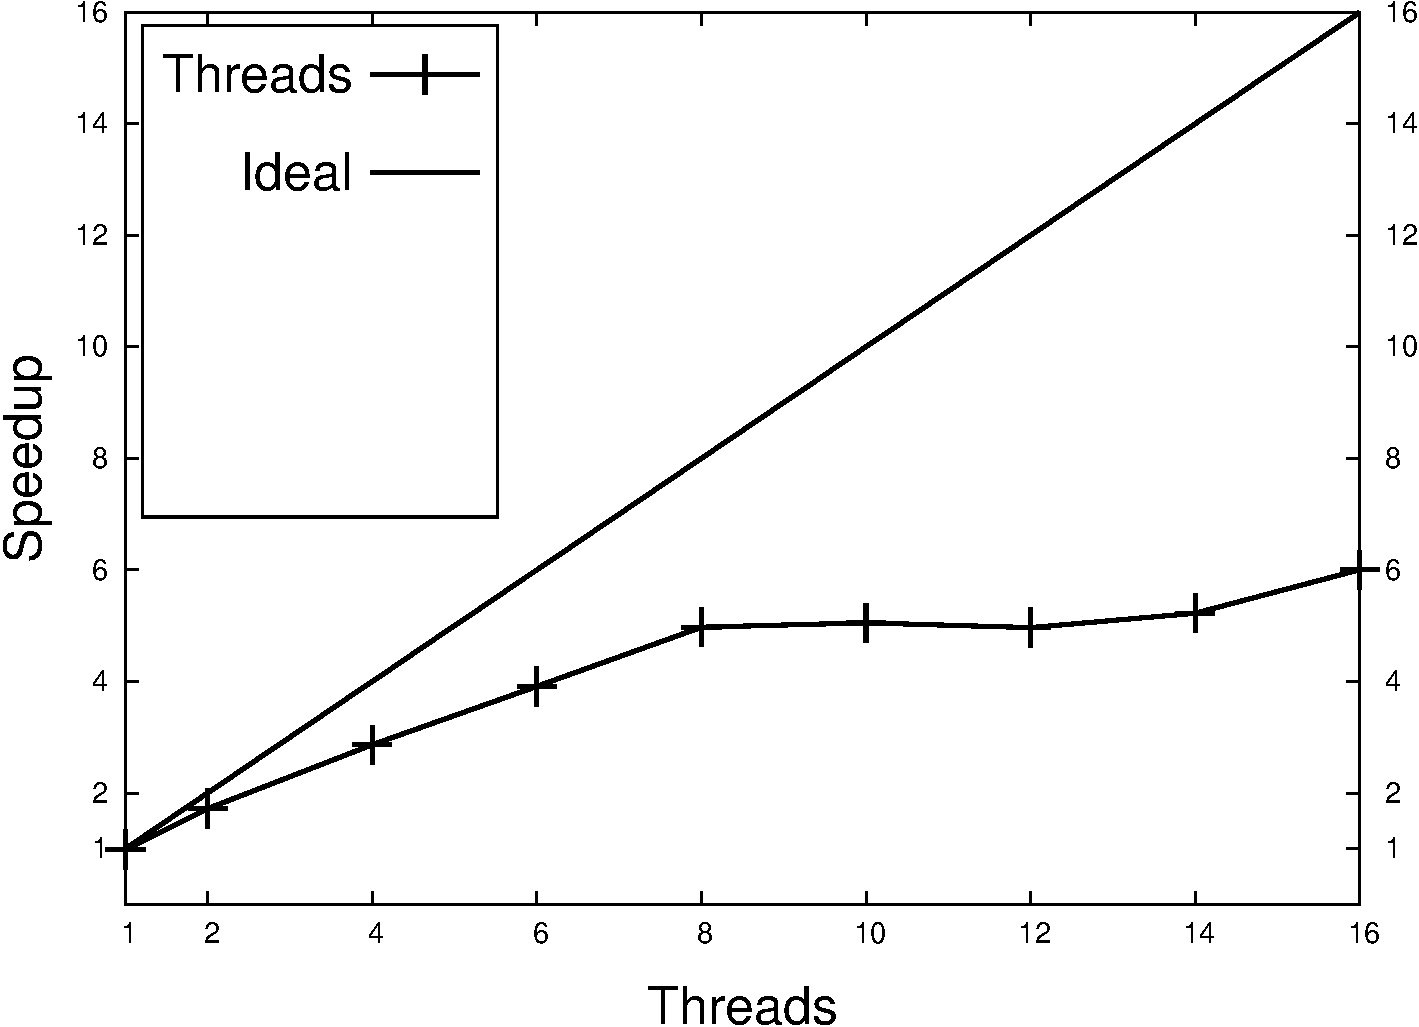
\includegraphics[width=0.5\textwidth]{speedup_pagerank-movies.pdf}}}
   \resizebox{\figsize}{!}{\subfigure[Using a random, dense graph (500 nodes)]{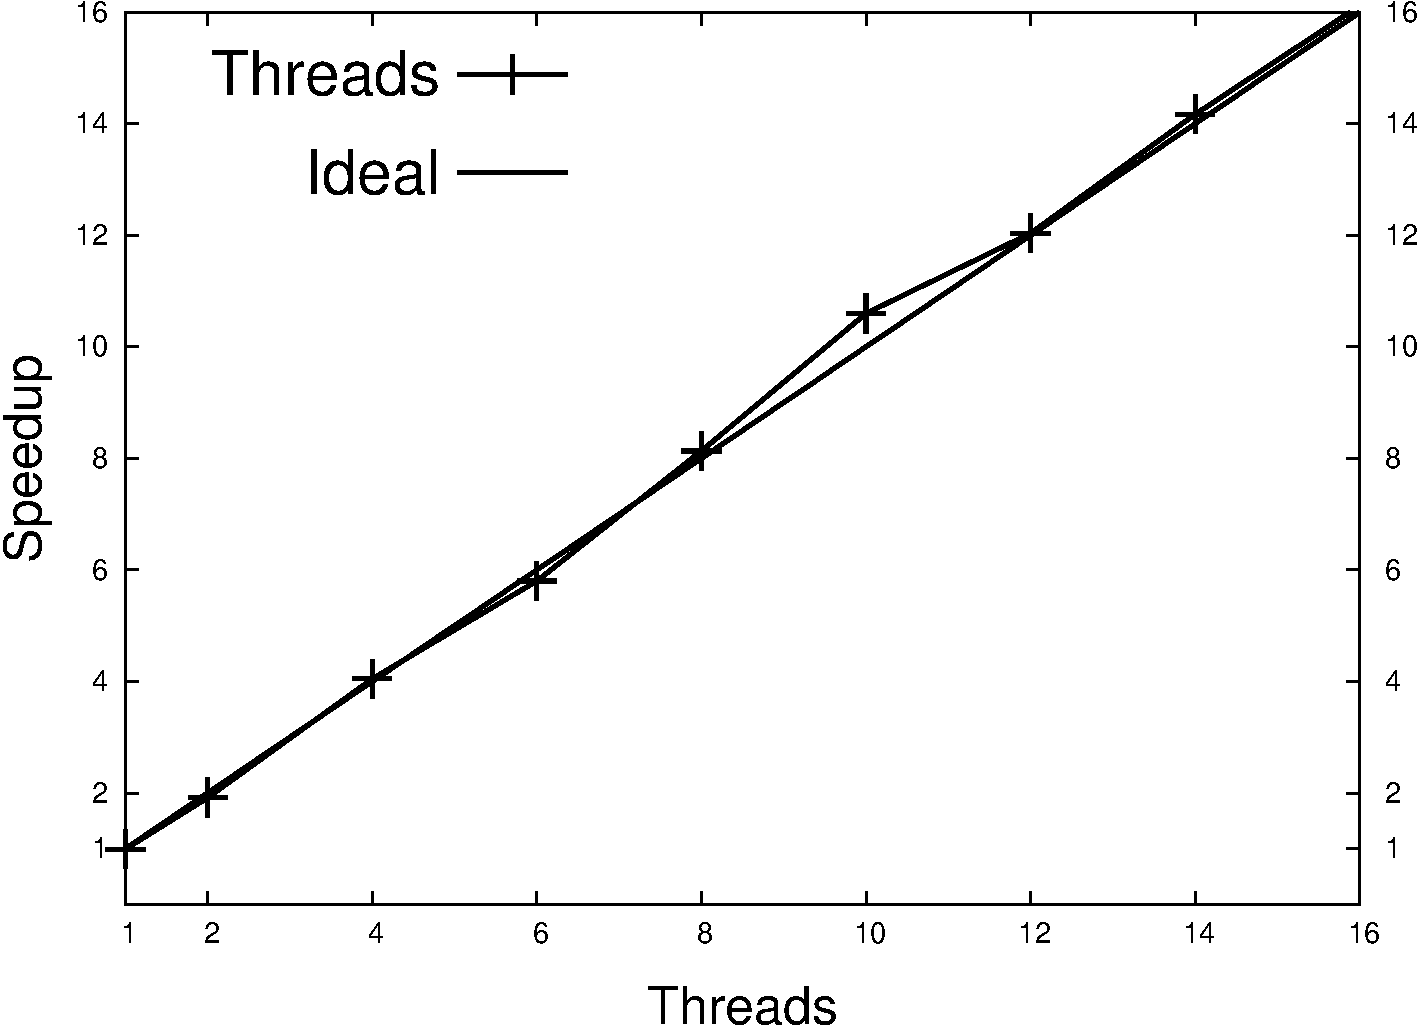
\includegraphics[width=0.5\textwidth]{speedup_pagerank-500.pdf}}}
   \caption{Experimental results for the asynchronous PageRank algorithm.}
   \label{exp:pagerank}
\end{figure*}

The PageRank results are shown in Fig.~\ref{exp:pagerank}. We have used the same web graph dataset as before and a new dataset representing movie websites \footnote{Both the search engine and movie web graphs were retrieved from \url{http://www.cs.toronto.edu/~tsap/experiments/download/download.html}}. We notice that the search engine graph dataset is big enough to allow good execution improvements even with 16 threads, while the movie graph, being smaller, shows some scaling problems as the number of threads increases. Even though the web graph follows the power law it does not slowdown execution (it happened in the graph coloring algorithm).
For the third plot, we used a random graph with about 500 nodes and 75000 edges. Since the graph is so dense, the runtime is capable of exploiting the
available parallelism, resulting in linear scalability.

\begin{figure}[h!]
     \centering
   \resizebox{\figsize}{!}{

    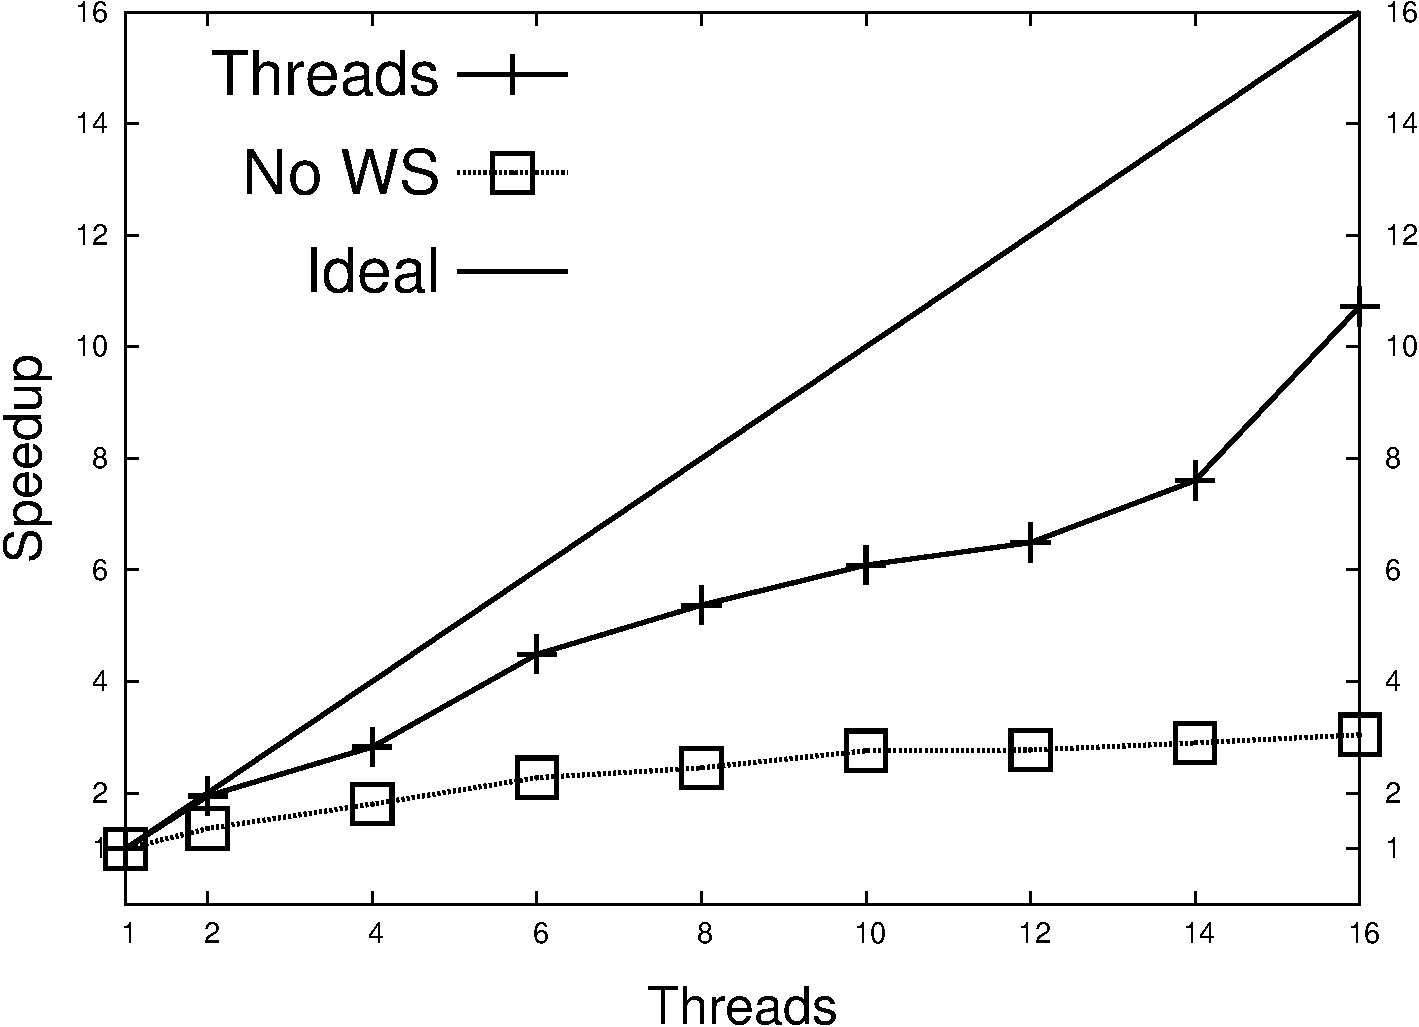
\includegraphics[width=0.5\textwidth]{speedup_8queens-11.pdf}}
    \caption{Experimental results for the N queens program (11x11~board).}
    \label{exp:8queens}
\end{figure}

The results for the N queens program are shown in Fig.~\ref{exp:8queens}. This program is much less regular than the other two, since computation starts at the top of the grid and then rolls down, until only the last row is doing computation. Note that as the computation goes from row to row, the number of states increase, creating even more imbalances. This shows that our system is able to scale well with more traditional algorithms such as N Queens.

\subsection{Coordination Experiments}

In our coordination experiments, we are interested in showing that coordination improves the execution time of programs.
To do this, we are using the following 3 programs:

\begin{description}
   \item[heat transfer]: In the heat transfer program, we have a grid of cells that transfer heat with the neighbor cells by taking into account the edge weights. We use a dataset with a square of cells in the center of the grid with very high heat, while the outer cells have low heat. We use coordination to prioritize the neighbors of cells where rapid heat changes happen.
   \item[shortest path]: We use the SSSP program shown earlier but we extended it to compute the distance to several nodes in order to increase the amount of computation.
   \item[belief propagation]: This is the program explained in the programs section. We build splash trees to improve performance.
\end{description}

Fig.~\ref{exp:heat-transfer} shows the results for the heat transfer program. \textbf{Threads} represents the speedup of the multicore execution
without coordination, while \textbf{Coord} represents the speedup when using coordination directives.
Both execution modes were compared against the sequential execution without coordination.
When using one thread, the coordinated version is almost 2 times
faster, however this speedup is slightly reduced as more threads are added. We think this happens because the \textbf{add-priority} action fact is ignored
when it is sent to a node located in a different thread.
Also note how the \textbf{Coord} line goes over the \textbf{Ideal} line, to the point where using 2 threads is 4 times faster when compared to a sequential
version without priorities.

\begin{figure}[h!]
     \centering
   \resizebox{\figsize}{!}{
   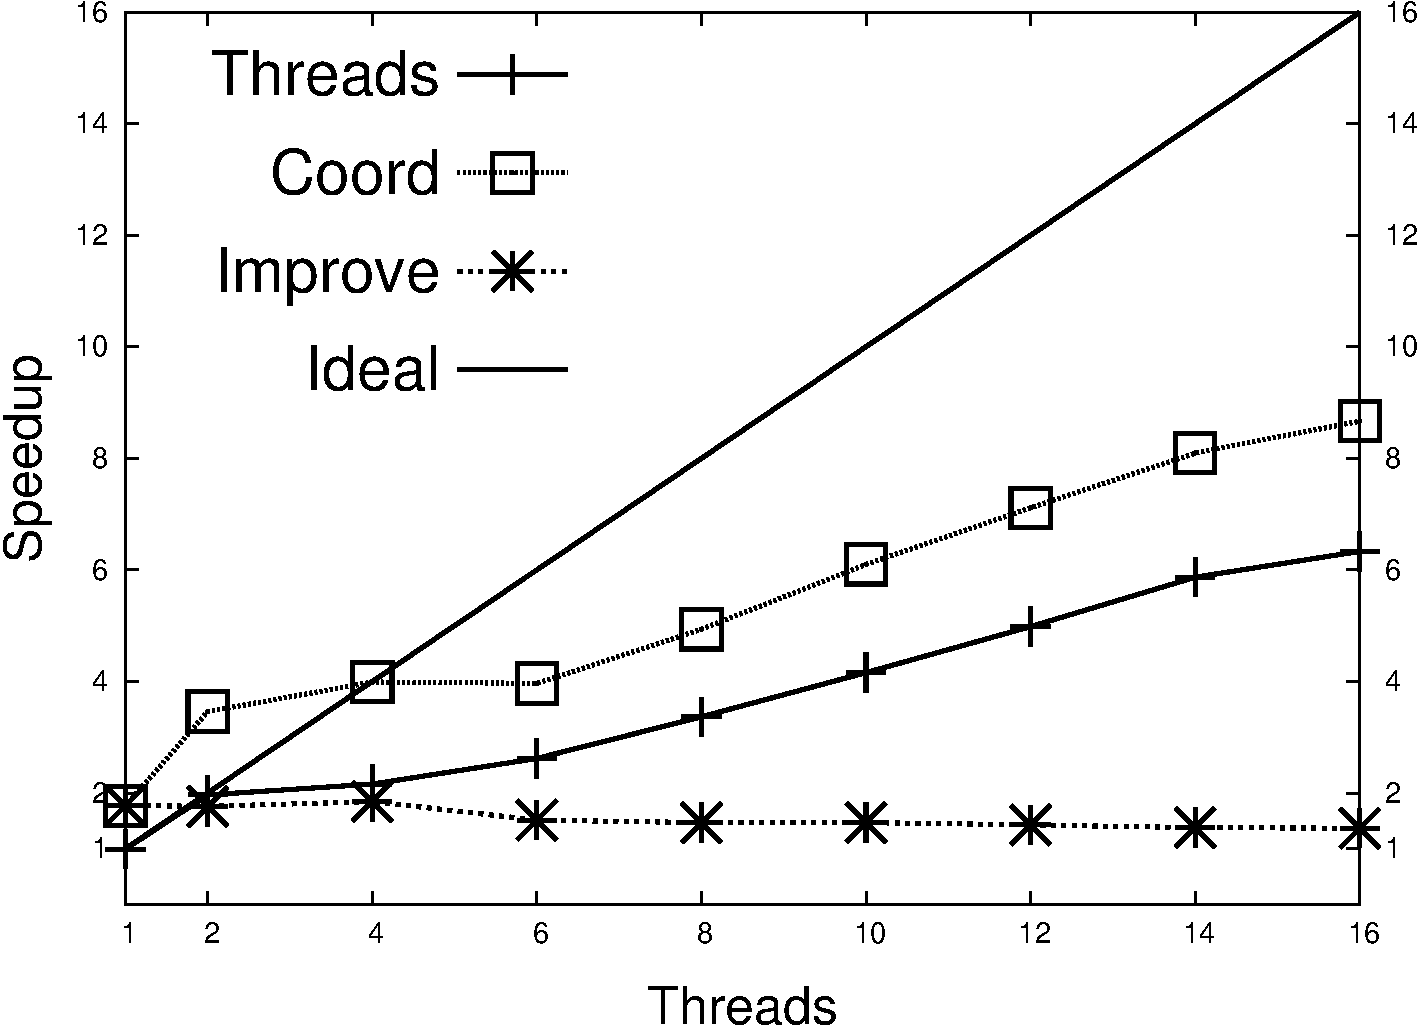
\includegraphics[width=0.5\textwidth]{speedup_heat-transfer-80.pdf}}
   \caption{Experimental results for the heat transfer program.}
   \label{exp:heat-transfer}
\end{figure}

To measure the performance of the SSSP program we used several datasets retrieved from \url{http://toreopsahl.com/datasets}. We computed several
statistics about each dataset, including: the number of nodes (\textbf{\# Nodes}), the number of edges (\textbf{\# Edges}) and
the average number of edges per node (\textbf{Edges / Node}). We also sorted the nodes by number of edges and counted the top number of nodes
with 25\% (\textbf{25\% Edges}), 50\% (\textbf{50\% Edges}) and 75\% (\textbf{75\% Edges}) of all edges.
These statistics and the speedup (\textbf{Speedup}) when using the coordinated version with 1 thread are presented in Table~\ref{tbl:shortest_path_speedup}.

We have tried to understand if there is a correlation between the graph structure and the coordination speedup. We can see that a higher number
of nodes and edges tends to improve execution. The US Airports dataset stands out because it is a small sized graph where a subset of airports
(70) have most connections. The other smaller datasets have a much stable distribution.
Still, the coordinated execution for most datasets is 30\% faster than the regular execution. We also included the speedup plot of the coordinated version
for the US Power Grid dataset in Fig.~\ref{exp:sssp-uspowergrid} that compares against the sequential execution without coordination.

\begin{table*}[ht]

\begin{center}
    \begin{tabular}{| l | c | c | c | c | c | c | c |}
    \hline
    \textbf{Dataset} & \textbf{Speedup} & \textbf{\# Nodes} & \textbf{\# Edges} & \textbf{Edges / Node} & \textbf{25\% Edges} & \textbf{50\% Edges} & \textbf{75\% Edges} \\ \hline \hline
    500 US Airports & 1.497 & 500 & 5960 & 11.92 & 14 & 37 & 70 \\ \hline
    US Power Grid & 1.459 & 4941 & 13188 & 2.67 & 485 & 1374 & 2131 \\ \hline
    Celegans Neural Network & 1.074 & 297 & 2345 & 7.89 & 24 & 65 & 104 \\ \hline
    Facebook like social network & 1.570 & 1899 & 20296 & 10.68 & 42 & 150 & 273 \\ \hline
    Intra-organizational network & 1.090 & 77 & 2288 & 28.94 & 9 & 24 & 36 \\ \hline
    \end{tabular}
\end{center}
     \caption{Summarized information about the datasets used in the SSSP program.}
     \label{tbl:shortest_path_speedup}
\end{table*}

\begin{figure}[h!]
     \centering
   \resizebox{\figsize}{!}{
   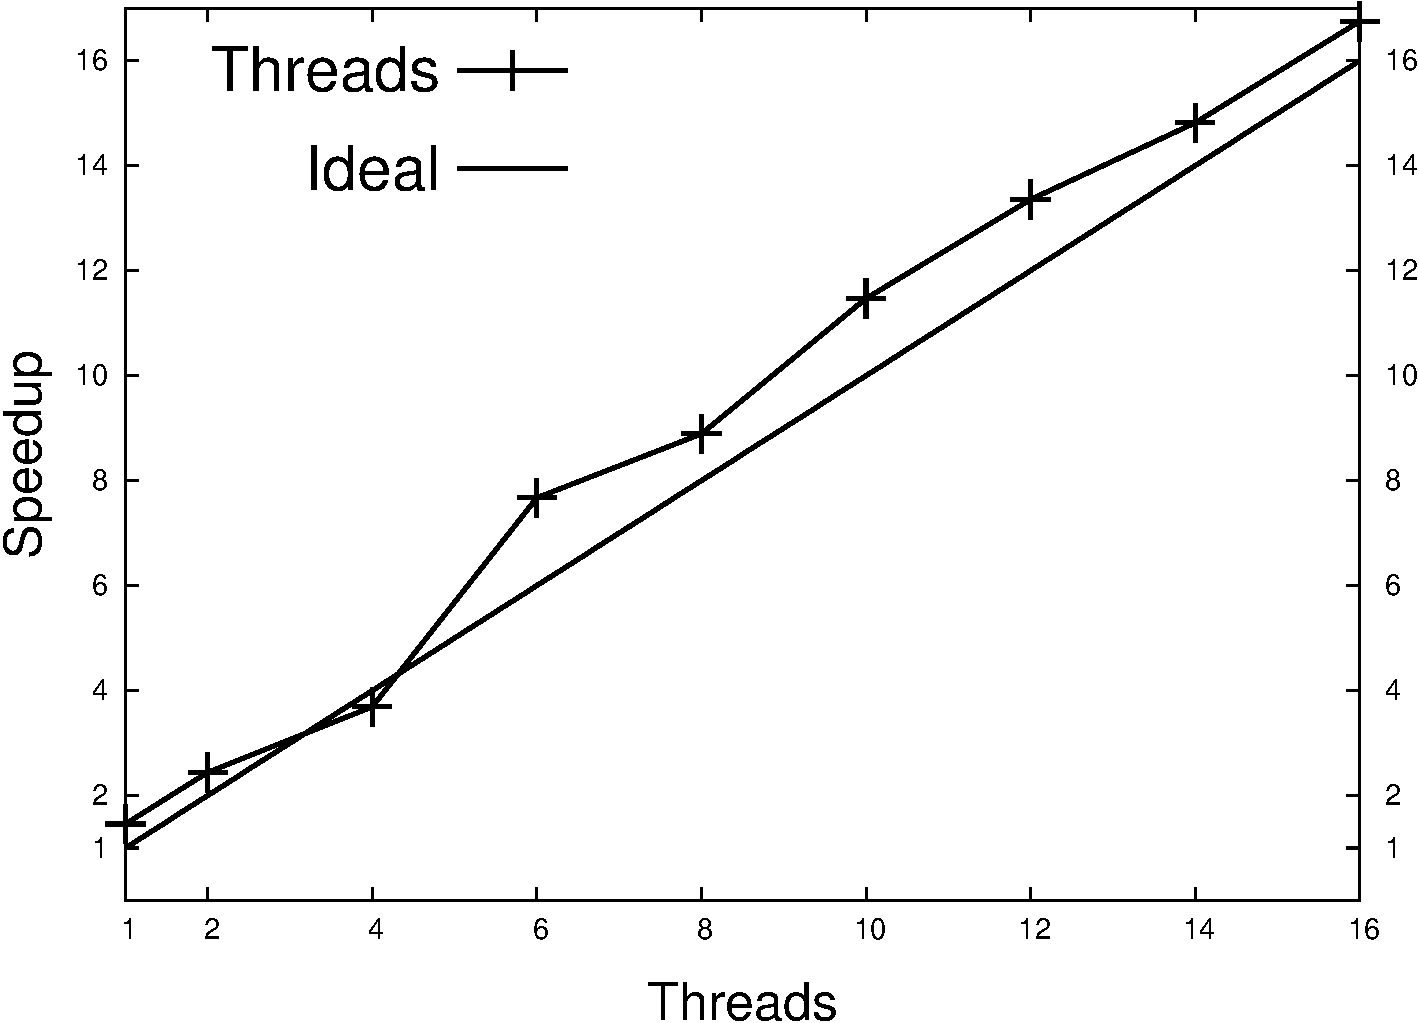
\includegraphics[width=0.5\textwidth]{speedup_uspowergrid.pdf}}
   \caption{Experimental results for the SSSP program with the US Power Grid dataset when using coordination.}
   \label{exp:sssp-uspowergrid}
\end{figure}

While the previous results were computed using only one thread, we also see good speedups with multiple threads. However, the gains reduce as we add
more threads because the decision of picking the best path is done at the thread level, thus reducing the opportunities for optimization.

For the belief propagation (BP) program, we have a noisy image made of 400x400 pixels that needs to be denoised.
To put our implementation to the test, we have also run the GraphLab (version 1) implementation of the same problem. The results are shown
in Fig.~\ref{exp:splashbp}. The first plot presents the scalability results for the simple belief propagation problem. The GraphLab version
uses the \textbf{fifo} scheduler that works identically to the basic \lang scheduler. While both versions show the same scalability pattern,
\lang runs about 3 to 4 times slower since it runs in a virtual machine, where GraphLab runs as a compiled C++ program.

\begin{figure*}[ht]
   \centering
   \resizebox{15cm}{!}{
   \subfigure[Scalability of basic belief propagation.]{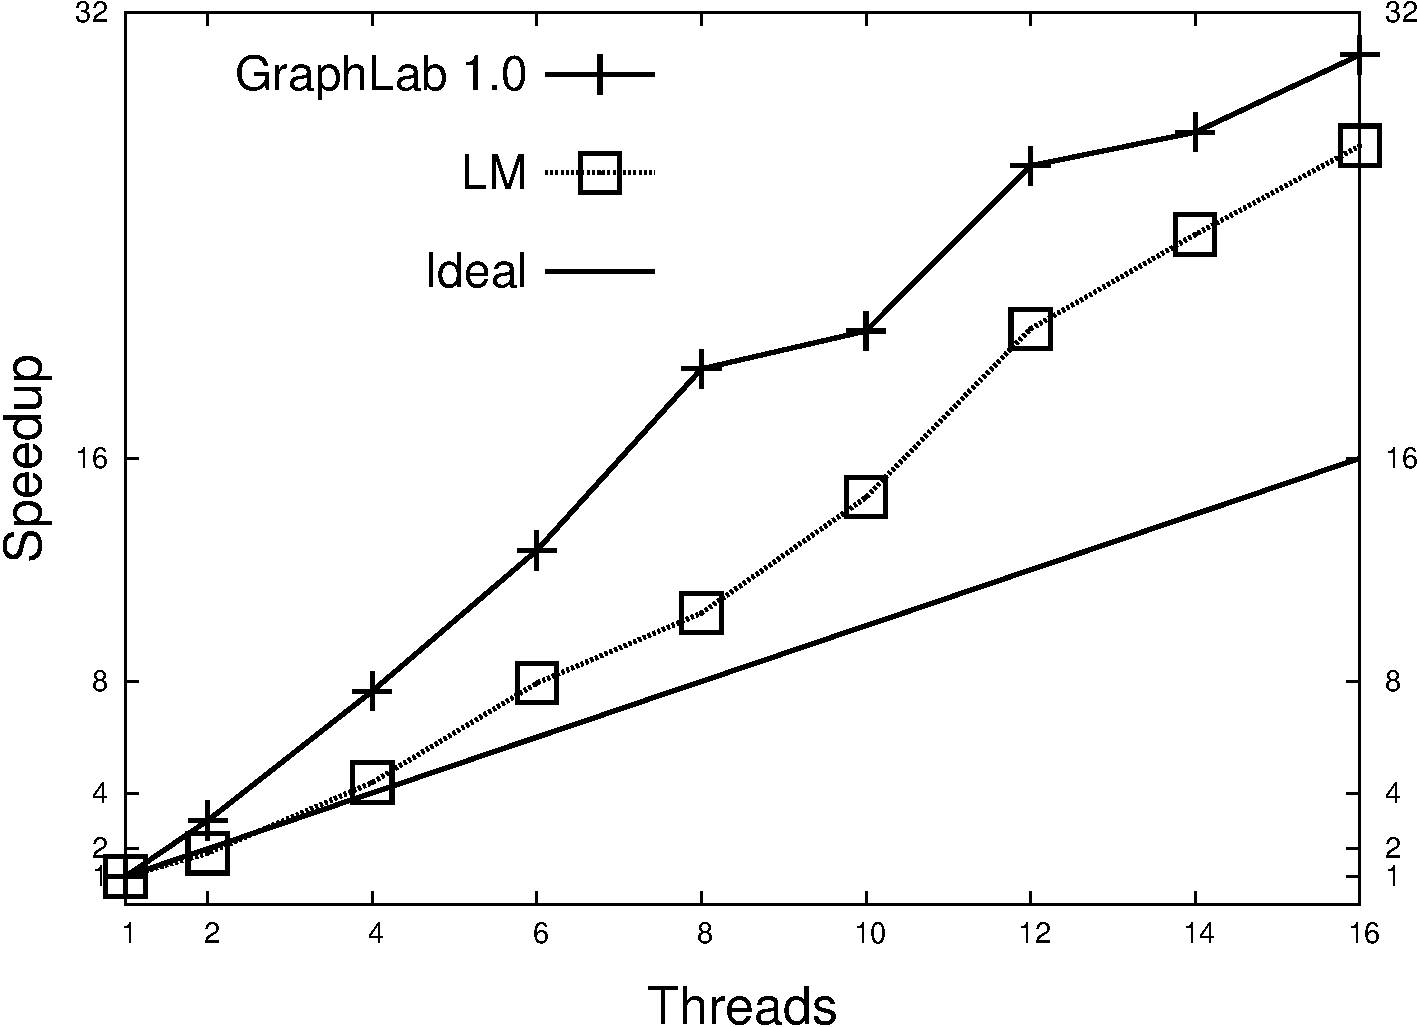
\includegraphics[width=0.7\textwidth]{splash-bp-speedup1_csv.pdf}}
   \subfigure[Scalability of belief propagation with splashes.]{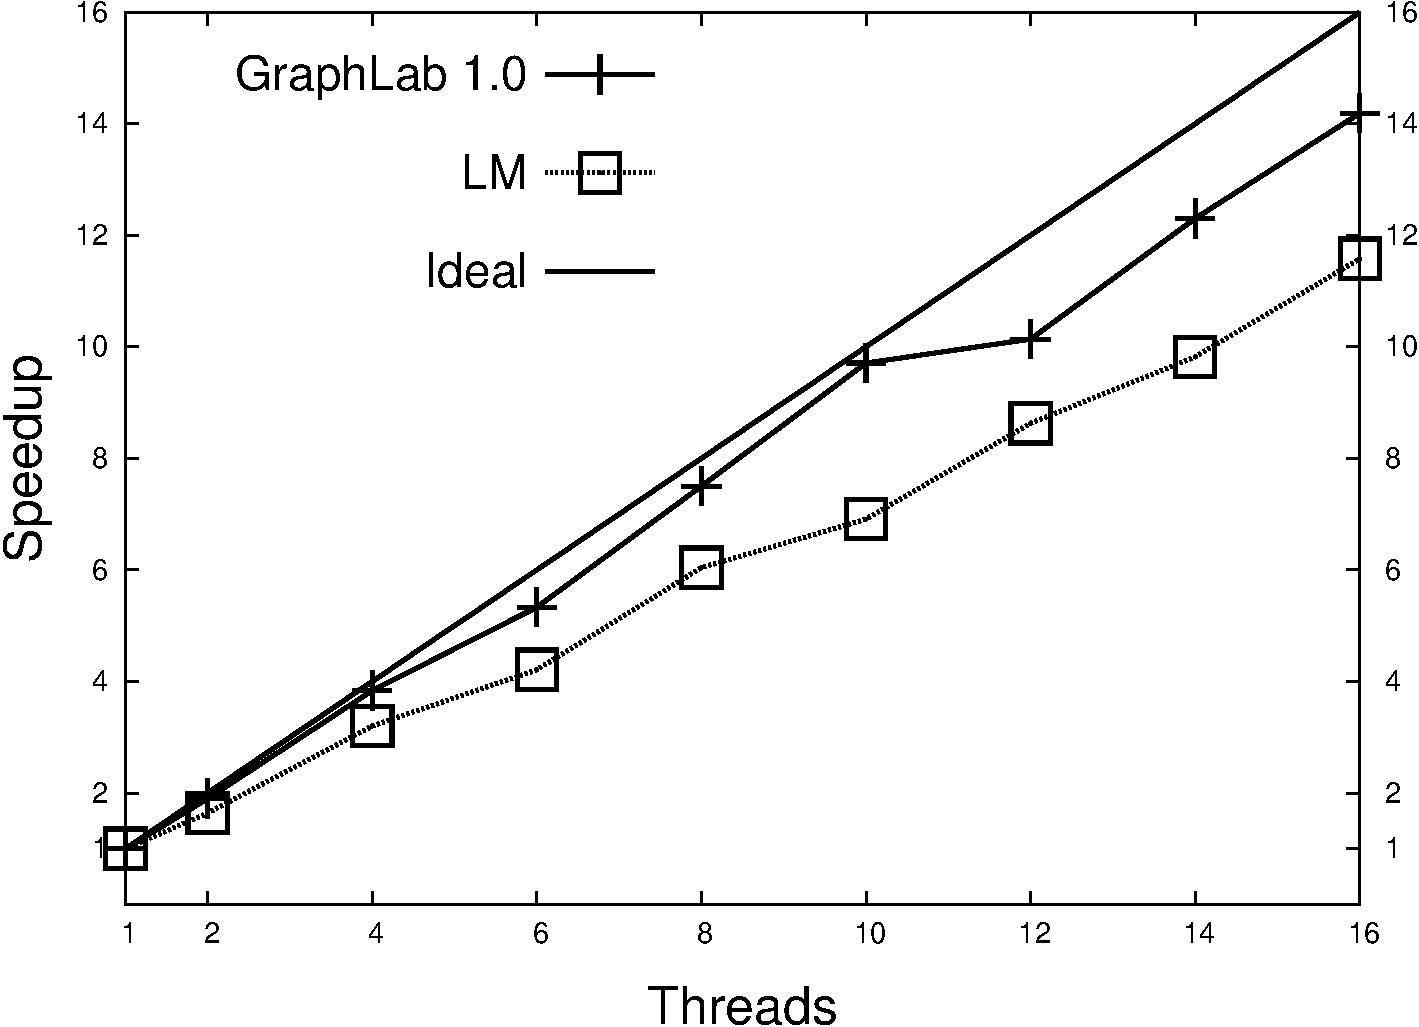
\includegraphics[width=0.7\textwidth]{splash-bp-speedup2_csv.pdf}}
   \subfigure[Coordination improvements by using splashes.]{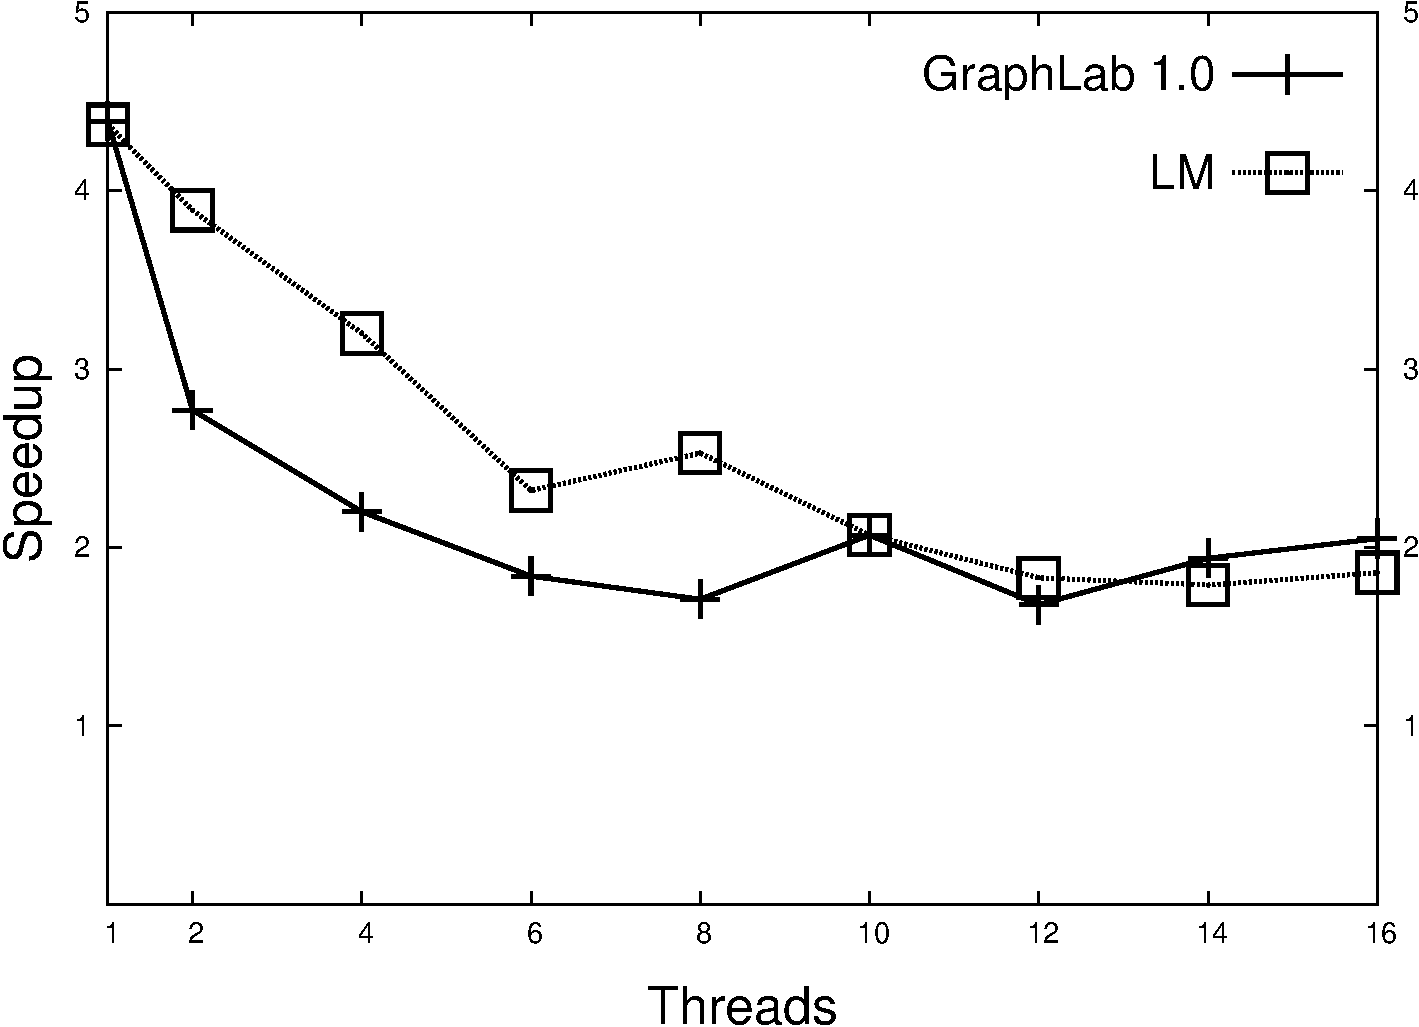
\includegraphics[width=0.7\textwidth]{splash-bp-improv_csv.pdf}}}
   \caption{Experimental results for belief propagation with coordination using splashes. The dataset is a 400x400 image.}
   \label{exp:splashbp}
\end{figure*}

The plot in Fig.~\ref{exp:splashbp}~(b) shows the scalability of the coordinated version. For GraphLab we used the \textbf{splash} scheduler, while \lang
runs with the extra coordination rules. Again, the scalability lines are very similar, but GraphLab appears to be slightly more scalable.
Finally, the last plot (Fig.~\ref{exp:splashbp}~(c)) presents the improvements of the coordinated version over the basic version when using a different
number of threads. We can see that adding more threads tends to reduce the effectiveness of splash trees in both systems.

The previous results validate our thesis that applying algorithm dependent scheduling strategies will make execution faster. By using a small set
of action facts and derivation rules we were able to implement complex scheduling strategies present in GraphLab, a practical and powerful machine learning
framework.

\subsection{Memory footprint}

In Fig.~\ref{tbl:memory} we present statistics for the memory footprint of the virtual machine. The data was taken right after the computation was completed
and it represents the memory allocated at that point, including facts and other auxiliary data structures.

\begin{table}[ht]
\begin{center}
      \resizebox{8.5cm}{!}{
    \begin{tabular}{| l | c | c | c | c | }
    \hline
    \textbf{Program} & \textbf{\# Nodes} & \textbf{\# Facts} & \textbf{Memory (MB)} & \textbf{Average (KB)} \\ \hline \hline
    N Queens & 121 & 3164 & 12.13 MB & 102.62 KB \\ \hline
    G. Graph Coloring web & 11659 & 1179671 & 293.06 MB & 25.74 KB \\ \hline
    %G. Graph Coloring weather & 8011 & 144927 & 43.78 MB & 5.60 KB \\ \hline
    PageRank web & 11659 & 1215580 & 309.78 MB & 27.20 KB \\ \hline
    %PageRank movie & 7967 & 147124 & 51.17 MB \\ \hline
    Heat transfer & 6400 & 44480 & 55.82 MB & 8.93 KB \\ \hline
    SSSP US Airports & 500 & 55960 & 16.87 MB & 34.54 KB \\ \hline
    %SSSP US Power Grid & 4941 & 502347 & 159.27 MB \\ \hline
    %BP & 160000 & 2395200 & 4408.48 MB \\ \hline
    Splash BP & 160000 & 2555200 & 2540.96 MB & 16.26 KB \\ \hline
    \end{tabular}}
\end{center}
     \caption{Memory usage of programs.}
     \label{tbl:memory}
\end{table}

In the \textbf{Average (KB)} column, we included the average memory used by a node computed by computing \textbf{Memory (MB)} / \textbf{\# Nodes}.
We note that, for the N Queens program, the average memory is quite high due the number of solutions (2680).
Surprisingly, the Splash BP program shows a low average memory usage even when taking into account the high number of lists used by the program
to store the belief values. In the future, we intend to bring these numbers down by optimizing the code, better fact storage and more efficient
data structures.

\subsection{Language expressiveness and conciseness}

We are also interested in measuring how long \lang programs are when compared to implementations of the same programs in other languages.
We want to show that \lang programs are more concise and can also be run in parallel from the start.

In table~\ref{tbl:length} we show how \lang programs against programs written in other languages in
terms of size. SSSP and the C version of N Queens~\cite{8queens-parallel} are sequential implementations and are difficult
to adapt to run in parallel. Even so, \lang programs are much smaller and in our opinion, easier
to understand. For the N Queens problem, we also included an MPI implementation written in C~\cite{Rolfe:2008:SMA:1473195.1473217}
that is around 10 times longer than the \lang version. We are currently developing an MPI version
of the \lang runtime and preliminary results show some good speedups for this program.

\begin{table}[ht]
\begin{center}
    \begin{tabular}{| c | c | l | c |}
    \hline
    \textbf{Program} & \textbf{\lang} & \textbf{Others} & \textbf{Average} \\ \hline \hline
    SSSP & 6 & 25 (C++) & 24\% \\ \hline
    PageRank & 30 & 60 (GraphLab) & 50\% \\ \hline
    BP & 50 & 90 (GraphLab) & 55\% \\ \hline
    Splash BP & 50 & 350 (GraphLab) & 14\% \\ \hline
    N Queens & 40 & 300 (C~\cite{8queens-parallel}), 400 (MPI~\cite{Rolfe:2008:SMA:1473195.1473217}) & 11\% \\ \hline
    \end{tabular}
\end{center}
     \caption{Comparison of source code size against other languages.}
     \label{tbl:length}
\end{table}

The GraphLab versions of PageRank, BP and Splash BP are all written in C++ and can be run in
parallel. We only counted the bare minimum number of lines for these programs (the update function)
so that our analysis is not biased towards \lang. The \lang versions of PageRank and BP are around
half of the size of the GraphLab versions. However, \lang really shines when we count the scheduling
code of the Splash BP program and compare it against the corresponding code of GraphLab. The \lang
version is far more concise.
